\mychapter{Background}{Background}{}\label{chap:background}

\section{Wastewater Treatment Works}
Municipal wastewater treatment plants purify our water using a series of steps. Large facilities typically rely on an effective biological method known as the activated sludge process. This system utilizes enormous tanks filled with beneficial microorganisms that naturally break down pollutants. During this process, the microorganisms convert the organic pollutants primarily into carbon dioxide, water, and new cellular biomass. These bacteria require a steady supply of oxygen to survive and work efficiently. To provide this air, facilities often use a technique called Fine Bubble Diffused Aeration (FBDA), which continuously pumps millions of tiny bubbles directly into the water. This happens in a part of the treatment plant known as\textbf{aerobic zones}. 

Once this active treatment is complete, the mixture flows into large circular settling tanks called \textbf{clarifiers}. The dense microbial biomass gradually settles to the bottom of the tank. This settling process leaves clear, treated water at the surface. Rather than discarding this settled biomass, the system continuously circulates it back to the initial tanks. Returning this activated sludge maintains a sufficient concentration of active microorganisms, ensuring the system can efficiently metabolize incoming organic matter.

Interestingly, someone who knows what to look for can tell a lot about how well these systems are performing just from aerial or satellite photos. A healthy FBDA unit churns the surface into a "leopard print" pattern, while a struggling one looks noticeably smoother. Clarifiers tell a similar story: when they are operating correctly, they separate out the solids and leave behind a clear liquid that looks black from above. When they are operating poorly, solids escape into the effluent and the surface turns green, cloudy, or uneven. Shown in Figure \ref{fig:treatment_comparison} are examples of functional and dysfunctional aerators and clarifiers, highlighting the visual cues that indicate their performance levels.

\begin{figure}[htbp]
    \centering 
    
    \begin{subfigure}[t]{0.31\textwidth}
        \centering
        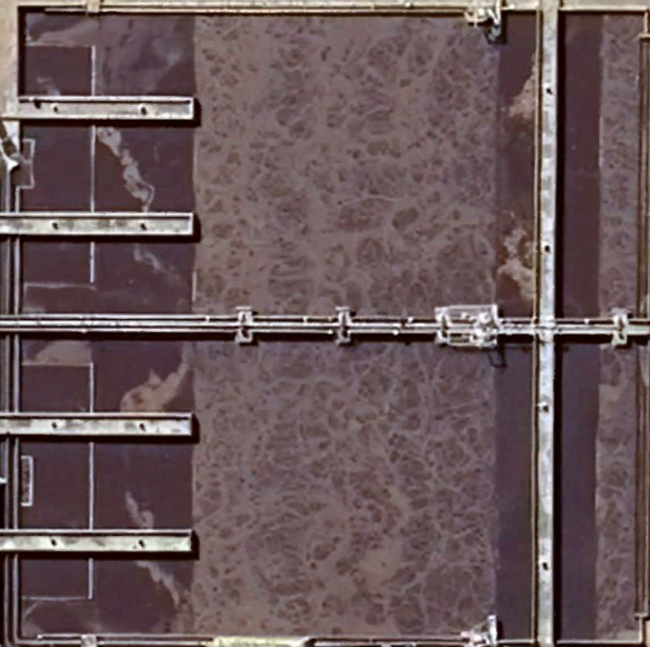
\includegraphics[width=\textwidth]{figures/aerobicfunc_background.png}
        \caption{Example of a functional aerator characterized by its "leopard print" pattern.}\label{fig:aerobic_func}
    \end{subfigure}
    \hfill
    \begin{subfigure}[t]{0.31\textwidth}
        \centering
        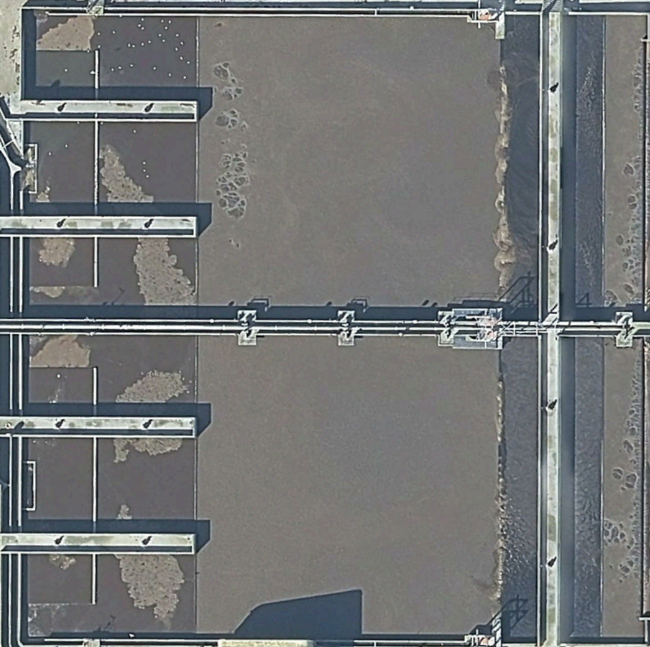
\includegraphics[width=\textwidth]{figures/aerobicdysfunc_background.png}
        \caption{Example of a dysfunctional aerator with a smooth surface, indicating poor performance.}\label{fig:aerobic_dysfunc}
    \end{subfigure}
    \hfill
    \begin{subfigure}[t]{0.31\textwidth}
        \centering
        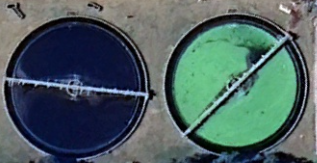
\includegraphics[width=\textwidth]{figures/clarifier_background.png}
        \caption{Functional clarifier on the left, dysfunctional clarifier on the right. The functional clarifier has a clear surface, while the dysfunctional one has solids floating on top.}\label{fig:clarifier}
    \end{subfigure}
    
    \caption{Visual comparison of functional and dysfunctional wastewater treatment components.}\label{fig:treatment_comparison}
\end{figure}
\section{Convolutional Neural Networks}
TODO


